\documentclass[tikz, border=10pt]{standalone}
\usepackage{amsmath}
\usepackage{xcolor}
\usetikzlibrary{arrows.meta, calc}

\definecolor{green1}{RGB}{0, 150, 80}

\begin{document}

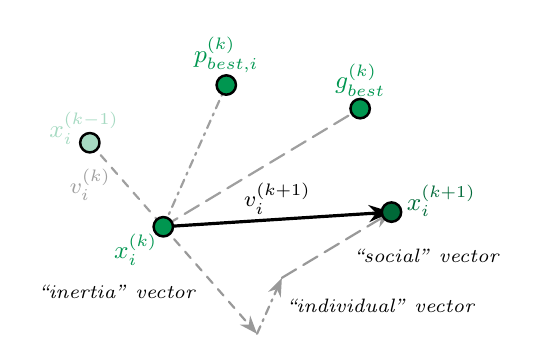
\begin{tikzpicture}[
    >=Stealth,
    line cap=round,
    line join=round,
    every node/.style={font=\small},
    point/.style={circle, draw=black, line width=0.9pt, minimum size=7pt, inner sep=0pt},
    guide/.style={dashed, gray!75, line width=0.8pt},
    vector/.style={->, black, line width=1.15pt},
    component/.style={->, gray!80, dashed, line width=0.8pt}
]

\coordinate (previous) at (0.717, 1.417);
\coordinate (current) at (1.65, 0.35);
\coordinate (personal) at (2.45, 2.15);
\coordinate (global) at (4.15, 1.85);
\coordinate (next) at (4.548, 0.536);
\coordinate (inertia-end) at (2.84, -1.01);
\coordinate (individual-end) at (3.156, -0.299);
\coordinate (social-end) at (5.05, 0.05);

\draw[guide] (previous) -- node[left=2pt, font=\footnotesize] {$v_i^{(k)}$} (current);
\draw[guide, dash dot] (current) -- (personal);
\draw[guide, dash pattern=on 6pt off 3pt] (current) -- (global);
\draw[component] (current) -- (inertia-end);
\draw[component, dash dot] (inertia-end) -- (individual-end);
\draw[component, dash pattern=on 6pt off 3pt] (individual-end) -- (next);

\draw[vector] (current) -- node[above=0pt, yshift=-2pt, font=\footnotesize] {$v_i^{(k+1)}$} (next);

\node[point, fill=green1!35!white] at (previous) {};
\node[point, fill=green1] at (current) {};
\node[point, fill=green1] at (personal) {};
\node[point, fill=green1] at (global) {};
\node[point, fill=green1!70!black] at (next) {};

\node[above left=-4pt, xshift=10pt, yshift=0pt, text=green1!35!white] at (previous) {$x_i^{(k-1)}$};
\node[below=3pt, xshift=-10pt, yshift=4pt, text=green1] at (current) {$x_i^{(k)}$};
\node[above=1pt, text=green1] at (personal) {$p_{best,i}^{(k)}$};
\node[above=1pt, text=green1] at (global) {$g_{best}^{(k)}$};
\node[right=2pt, yshift=4pt, text=green1!70!black] at (next) {$x_i^{(k+1)}$};

\node[left=2pt, yshift=-4pt, font=\scriptsize\itshape] at ($(current)!0.5!(inertia-end)$) {``inertia'' vector};
\node[right=2pt, font=\scriptsize\itshape] at ($(inertia-end)!0.5!(individual-end)$) {``individual'' vector};
\node[right=2pt, yshift=-4pt, font=\scriptsize\itshape] at ($(individual-end)!0.5!(next)$) {``social'' vector};

\end{tikzpicture}

\end{document}
